\documentclass[conference]{IEEEtran}
\IEEEoverridecommandlockouts

\usepackage{cite}
\usepackage{amsmath,amssymb,amsfonts}
\usepackage{graphicx}
\usepackage{textcomp}
\usepackage{xcolor}
\usepackage{booktabs}
\usepackage{array}
\usepackage{tabularx}
\usepackage{multirow}
\usepackage{tikz}
\usetikzlibrary{arrows.meta,positioning,calc,shapes.geometric}
\usepackage[hidelinks]{hyperref}

\definecolor{nyx}{HTML}{5B4BD6}
\definecolor{nyx2}{HTML}{0F9D8A}
\newcolumntype{Y}{>{\raggedright\arraybackslash}X}
\newcolumntype{L}[1]{>{\raggedright\arraybackslash}p{#1}}

\begin{document}

\title{NyxChain: A Layer-1 Blockchain with Reliability-Weighted Proof of Stake and Bounded Voting Power}

\makeatletter
\newcommand{\linebreakand}{%
  \end{@IEEEauthorhalign}
  \hfill\mbox{}\par
  \mbox{}\hfill\begin{@IEEEauthorhalign}
}
\makeatother

\author{
\IEEEauthorblockN{\textbf{Mukkara Rithvik Reddy}}
\IEEEauthorblockA{\textit{Dept. of Computer Science and Engineering}\\
\textit{Amrita School of Computing}\\
Amrita Vishwa Vidyapeetham, Bengaluru, India\\
bl.en.u4cse23264@bl.students.amrita.edu}
\and
\IEEEauthorblockN{\textbf{Aman Aggarwal}}
\IEEEauthorblockA{\textit{Dept. of Computer Science and Engineering}\\
\textit{Amrita School of Computing}\\
Amrita Vishwa Vidyapeetham, Bengaluru, India\\
bl.en.u4cse23206@bl.students.amrita.edu}
\linebreakand
\IEEEauthorblockN{\textbf{Harsh Vardan Singh}}
\IEEEauthorblockA{\textit{Dept. of Computer Science and Engineering}\\
\textit{Amrita School of Computing}\\
Amrita Vishwa Vidyapeetham, Bengaluru, India\\
bl.en.u4cse23222@bl.students.amrita.edu}
}

\maketitle

\begin{abstract}
Proof-of-stake blockchains replace the computational lottery of proof of work with an economic one, but in doing so they allow influence over block production and finality to be acquired instantly by purchase, and they offer no protection against a single participant accumulating a decisive share of the vote. Reputation-based designs make influence slow to acquire, yet in existing formulations reputation accumulates without bound, so that trust earned early continues to count indefinitely and carries no economic penalty for misbehaviour. This study presents NyxChain, a Layer-1 blockchain implemented from first principles, comprising its own block and transaction formats, peer-to-peer network, mempool, wallet and live block explorer, in which these two shortcomings are addressed jointly. Validator weight is the product of stake and reputation, where reputation is defined as \emph{recent reliability}: an exponentially weighted moving average over on-chain-verifiable duties (timely finality votes and block proposals) with a half-life of approximately 50 blocks. Validators performing identical work therefore converge to identical reputation irrespective of when they joined, and a validator that ceases to participate loses its standing within a few dozen blocks. A voting-weight cap limits any single validator to 30\% of total weight, subject to a boost limit under which no other validator's share is ever more than doubled. Blocks become irreversible once votes representing two thirds of total weight are recorded on chain, and equivocation is punished by evidence-based slashing. On a four-validator network with one-second slots, the implementation passes 30 unit tests, a 20-check end-to-end scenario and a 9-check Byzantine scenario; it sustains 446--509 transfers per second, finalizes blocks a median of 1.0\,s after they appear, continues to finalize while a validator or an offline participant holding 18 times the stake of a regular validator is absent, and restores a crashed validator to synchronization 0.71\,s after restart. An independent code review identified one design flaw in an earlier formulation of the cap, which is described and corrected.
\end{abstract}

\begin{IEEEkeywords}
Blockchain, proof of stake, reputation-based consensus, Byzantine fault tolerance, finality, slashing, Sybil resistance, peer-to-peer networks, distributed ledgers.
\end{IEEEkeywords}

%=====================================================================
\section{Introduction and Background}

A blockchain allows parties that do not trust one another to agree on a single, append-only history of transactions without a central operator. The property is not obtained for free: every design must decide how participants discover one another, which participant may extend the history at a given moment, what prevents one entity from impersonating many, and when an entry may be regarded as permanent.

\subsection{From Computational to Economic Consensus}
Bitcoin resolved these questions by requiring a proposer to solve a computational puzzle and by treating the longest chain as authoritative \cite{nakamoto2008}. The arrangement removes the need for a known participant list, but it consumes energy in proportion to the security it provides and offers only probabilistic finality: a block becomes less likely to be reverted as more blocks are built on it, but never impossible to revert. Subsequent analysis formalized its guarantees \cite{garay2015} and showed that the reward mechanism is not incentive-compatible, since a colluding minority can earn more than its share by withholding blocks \cite{eyal2014}.

Proof-of-stake protocols replace computational work with locked economic deposits. Ouroboros \cite{kiayias2017}, Ouroboros Praos \cite{david2018} and Algorand \cite{gilad2017} demonstrated that stake can serve as the Sybil-resistance mechanism with security guarantees comparable to those of proof of work, and finality gadgets such as Casper FFG \cite{buterin2017} and pipelined Byzantine-fault-tolerant protocols such as HotStuff \cite{yin2019} added deterministic irreversibility.

\subsection{The Influence Problem}
Under proof of stake, influence is proportional to holdings at the moment of measurement. Three consequences follow:
\begin{itemize}
\item \textbf{Instant acquisition.} A participant who purchases a large stake receives the corresponding voting power immediately, with no record of honest behaviour.
\item \textbf{Concentration.} No mechanism prevents a single participant from holding a share of the vote large enough to stall finality by abstaining, which requires only one third of total weight.
\item \textbf{Indifference to reliability.} A validator that is frequently offline retains its full weight, so the network continues to wait on it.
\end{itemize}
Reputation-based designs \cite{yu2019,aluko2021} address the first consequence by making influence depend on behaviour observed over time. In the existing formulations, however, reputation grows by accumulation: trust earned early continues to count indefinitely, so that early participants retain a lasting advantage over later participants performing identical work, and a participant with a long record may cease to contribute while retaining its standing.

\subsection{Relevance}
The questions above are not confined to public cryptocurrencies. Consortium ledgers, inter-institutional record systems and campus-scale deployments face the same choice of who may write, how quickly a write becomes final, and what prevents one member from dominating. A design in which influence must be earned, fades when it is no longer earned, and is bounded for any single member is directly applicable to such settings.

\subsection{Design Objectives}
The system was built against the targets in Table~\ref{tab:targets}, each chosen to reflect a property that a reviewer of a consensus protocol would check first.

\begin{table*}[t]
\centering
\caption{Operational Targets and Achieved Values}
\label{tab:targets}
\small
\begin{tabularx}{\textwidth}{@{}L{3.1cm} L{3.4cm} L{3.9cm} Y@{}}
\toprule
\textbf{Objective} & \textbf{Target} & \textbf{Achieved} & \textbf{Justification}\\
\midrule
Finality latency & Final within two slots of appearing & Median 1.0\,s, max 2.0\,s with 1\,s slots (met) & Users need to know when a payment can no longer be reversed.\\
Throughput & $\geq$ 400 transfers/s on one machine & 446--509 transfers/s (met) & Demonstrates that validation, not the network, bounds the design.\\
Crash tolerance & Finality continues with 1 of 4 validators offline & +18 finalized heights in 20 slots (met) & A single failed machine must not halt the ledger.\\
Recovery & Restarted validator in sync within 5\,s & 0.71\,s (met) & Short outages should not require operator intervention.\\
Accountability & Equivocation slashed within 2 blocks & Proof on chain in the next block (met) & Safety must rest on an economic penalty, not on goodwill.\\
Instant influence & Newcomer weight $\leq$ 1/5 of a genesis validator with equal stake & Joins at 10\% vs 50\% reputation (met) & Voting power must not be purchasable at once.\\
Fairness of reputation & Spread $\leq$ 5 points among validators doing equal work & 1.8 points (met) & Early arrival must not confer a lasting advantage.\\
Concentration & Single validator $\leq$ 30\% of the vote & Met while it holds $<$ 65\% of raw weight; loosens above (partially met) & Below one third, no single validator can stall finality alone.\\
\bottomrule
\end{tabularx}
\end{table*}

The contributions of the present work are as follows. (i) A complete, from-scratch Layer-1 implementation, including networking, persistence, wallet and explorer, in approximately 2{,}050 lines of protocol code with a single cryptographic dependency. (ii) A definition of reputation as recent reliability, under which reputation is a bounded, self-correcting score rather than an accumulating quantity. (iii) A voting-weight cap with an explicit boost limit, which bounds a dominant validator without transferring disproportionate power to small or unreliable validators. (iv) An evaluation in which every reported figure is produced by a script that exits with a failure status if its check is not met, with full logs retained.

%=====================================================================
\section{Material and Experimental Environment}
This section describes the software platform, the network configurations, the workloads, and the fault and attack scenarios under which all subsequent results are obtained. No external blockchain, framework or database is used, and every experiment is reproducible from the public repository.

\subsection{Software Platform}
The implementation is written in Python 3. Its only dependency outside the standard library is the \texttt{cryptography} package, which supplies Ed25519 signatures; hashing uses SHA-256. Nodes communicate over TCP with newline-delimited JSON messages, persist accepted blocks to an append-only file, and expose an HTTP interface that serves both a JSON API and a browser dashboard. Experiments were run on a single host with two CPU cores; all nodes therefore share one machine and network latency is close to zero.

\subsection{Network Configurations}
Each experiment generates a fresh network, consisting of key pairs, a genesis document and per-node configuration, with the genesis time set a few seconds in the future so that every node starts from slot zero. Table~\ref{tab:configs} lists the configurations. Each node is given the address of a single seed peer and must discover the remainder through peer exchange.

\begin{table}[t]
\centering
\caption{Experimental Configurations}
\label{tab:configs}
\footnotesize
\begin{tabularx}{\columnwidth}{@{}L{1.6cm} L{1.9cm} Y@{}}
\toprule
\textbf{Experiment} & \textbf{Network} & \textbf{Purpose}\\
\midrule
Unit tests & In-process, simulated clock & Correctness of each rule in isolation (30 tests)\\
End-to-end demo & 4 validator processes, 1\,s slots & Payments, staking, crash and restart, reputation, whale (20 checks)\\
Attack demo & 4 validators, one Byzantine & Detection and slashing of equivocation (9 checks)\\
Reputation simulation & 5 validators, 300 blocks, simulated clock & Long-run reputation dynamics; cap response curve\\
Benchmark & 4 validators, 1\,s slots, 80 funded accounts & Throughput, finality latency, recovery time\\
\bottomrule
\end{tabularx}
\end{table}

\subsection{Workloads}
Two transaction loads are used in the benchmark. Load A consists of 1{,}000 signed transfers from 20 accounts (50 each); Load B consists of 4{,}000 transfers from 80 accounts. Transactions are signed in advance and submitted in batches spread evenly over the four nodes, so that propagation through the peer-to-peer layer is exercised. The end-to-end demonstration additionally issues ordinary transfers, a stake, a partial unstake, and a large stake by a participant that never operates a node.

\subsection{Fault and Attack Scenarios}
Four adverse conditions are exercised. \emph{Crash}: a validator process is terminated without warning and restarted later. \emph{Idle staker}: an account stakes but never runs a node, and therefore never votes or proposes. \emph{Whale}: an account stakes 9{,}000 tokens, eighteen times a regular validator's 500, and stays offline. \emph{Equivocation}: a validator, when selected, signs two different blocks for the same slot, sends each to a different half of the network, and votes for both.

\subsection{Measurement Procedure}
Every scenario is driven by a script that queries the nodes' APIs and evaluates explicit pass/fail checks; the script exits with a non-zero status if any check fails, so the scenarios also serve as integration tests. Finality latency is measured by polling one node every 50\,ms and recording, for each height, the first observation of the block and the first observation of its finality. Node logs, terminal outputs, dashboard screenshots and raw measurement data are retained for every run.

%=====================================================================
\section{Literature Survey, Comparison with Baseline Architectures and State-of-the-Art}
Consensus for open ledgers has developed along three largely separate lines: Nakamoto-style chains secured by work, stake-based protocols with formal guarantees, and Byzantine-fault-tolerant voting protocols that provide deterministic finality. Reputation-based designs form a smaller fourth line.

\subsection{Agreement Foundations}
Lamport, Shostak and Pease established that agreement in the presence of arbitrarily faulty participants requires more than two thirds of participants to be honest \cite{lamport1982}. PBFT made Byzantine replication practical for a fixed, known set of replicas under partial synchrony \cite{castro1999}, while Raft provided an understandable crash-fault-tolerant alternative based on leader election with randomized timeouts \cite{ongaro2014}. The two-thirds bound underlies every finality threshold that followed, including the one adopted here.

\subsection{Nakamoto Consensus and Fork Choice}
Bitcoin's longest-chain rule \cite{nakamoto2008} was formalized by Garay et al., who proved the common-prefix and chain-quality properties under an honest majority of computational power \cite{garay2015}. Eyal and Sirer showed that selfish mining lets a colluding pool exceed its fair share of rewards \cite{eyal2014}. Sompolinsky and Zohar demonstrated that the fork-choice rule is itself a security parameter, proposing the heaviest-subtree rule GHOST \cite{sompolinsky2015} and later a block-DAG generalization \cite{sompolinsky2018}. The weakness common to this line is that finality is only probabilistic.

\subsection{Provably Secure Proof of Stake}
Ouroboros was the first proof-of-stake protocol with security guarantees comparable to Bitcoin's, organizing time into epochs and slots with leaders elected by a secure coin-tossing procedure \cite{kiayias2017}. Ouroboros Praos extended this to semi-synchronous networks and adaptive corruption using verifiable random functions for private leader election \cite{david2018}. Algorand combined cryptographic sortition with a new Byzantine agreement protocol to confirm transactions within a minute without ordinary forks \cite{gilad2017}. In all three, influence is proportional to stake at the time of measurement, so it can be acquired at once by purchase.

\subsection{Byzantine-Fault-Tolerant Finality}
Casper FFG overlays a block-proposal mechanism with checkpoint votes and slashing conditions, so that safety is preserved even if proposal is attacked \cite{buterin2017}. HotStuff achieves responsiveness and linear communication during leader replacement through a chained, pipelined voting structure \cite{yin2019}. Both separate block production from finality and treat validator weight as given, rather than as something earned.

\subsection{Reputation-Based Consensus}
RepuCoin defines a miner's voting power by reputation integrated over the history of the chain, so that an attacker renting a temporary majority of hash power cannot control voting \cite{yu2019}; it remains built on proof of work. Proof-of-Reputation selects the consensus group from the highest-reputation nodes \cite{aluko2021} but has no stake at risk and no formal finality rule. In both, reputation increases by accumulation.

\subsection{Comparison with Baseline Architectures}
Table~\ref{tab:compare} consolidates the characteristics of the principal baselines.

\begin{table*}[t]
\centering
\caption{Comparison of Baseline and State-of-the-Art Consensus Architectures}
\label{tab:compare}
\footnotesize
\begin{tabularx}{\textwidth}{@{}l c L{2.6cm} L{2.6cm} L{2.2cm} L{2.0cm} Y@{}}
\toprule
\textbf{Protocol} & \textbf{Year} & \textbf{Sybil resistance / weight} & \textbf{How influence is acquired} & \textbf{Finality} & \textbf{Accountability} & \textbf{Bound on a single participant}\\
\midrule
Bitcoin \cite{nakamoto2008} & 2008 & Computation & Instantly, by buying hardware & Probabilistic & None & None\\
PBFT \cite{castro1999} & 1999 & Fixed replica set & Permissioned & Deterministic & None & Equal replicas\\
Ouroboros \cite{kiayias2017} & 2017 & Stake & Instantly, by buying stake & Probabilistic & None & None\\
Algorand \cite{gilad2017} & 2017 & Stake (sortition) & Instantly, by buying stake & Deterministic & None & None\\
Casper FFG \cite{buterin2017} & 2017 & Stake & Instantly, by buying stake & Deterministic (2 rounds) & Slashing & None\\
HotStuff \cite{yin2019} & 2019 & Fixed replica set & Permissioned & Deterministic & None & Equal replicas\\
RepuCoin \cite{yu2019} & 2019 & Work integrated over time & Slowly, accumulates without bound & Deterministic & Reputation loss & None\\
Proof-of-Reputation \cite{aluko2021} & 2021 & Reputation ranking & Slowly, accumulates & Not specified & Reputation loss & Group selection\\
\textbf{NyxChain} & 2026 & Stake $\times$ recent reliability & Slowly; fades when duties stop & Deterministic (1 round) & Slashing & 30\% cap, boost $\leq$ 2$\times$\\
\bottomrule
\end{tabularx}
\end{table*}

Two observations follow from Table~\ref{tab:compare}. First, every stake-based baseline grants influence at the moment of purchase, and none bounds the share of a single participant; the protocols that do bound it (PBFT, HotStuff) achieve this only by fixing the participant set in advance. Second, the reputation-based baselines make influence slow to acquire but never cause it to decay, so a participant's early record continues to count after its behaviour has changed.

\subsection{Identified Research Gaps}
\subsubsection{Gap 1 --- Influence can be bought instantly}
In stake-based protocols the voting power of a new participant is determined entirely by the size of its deposit. Among the stake-based designs surveyed, none requires a newcomer to demonstrate reliable behaviour before it obtains a material share of the vote.

\subsubsection{Gap 2 --- Reputation accumulates rather than reflects}
In the reputation-based designs examined, reputation is a running total. A validator that behaved well early retains an advantage over one that behaves identically but joined later, and a validator with a long record may stop participating while retaining its standing for an extended period. None of the designs surveyed defines reputation so that it reflects current reliability and so that identical behaviour yields identical reputation.

\subsubsection{Gap 3 --- Single-participant dominance is unbounded or bounded by flattening}
Open protocols place no limit on the share of the vote held by a single participant. A naive share cap transfers the excess weight to every other participant in proportion, which, when only one or two participants are large, hands decisive weight to the smallest or least reliable participants. None of the designs surveyed bounds the dominant participant while also bounding the amplification of the remainder.

%=====================================================================
\section{Methodology Architecture}

\subsection{System Overview}
Every node runs the same software; a validator node additionally holds a signing key and produces blocks and votes. Fig.~\ref{fig:arch} shows the layers of a node.

\begin{figure}[t]
\centering
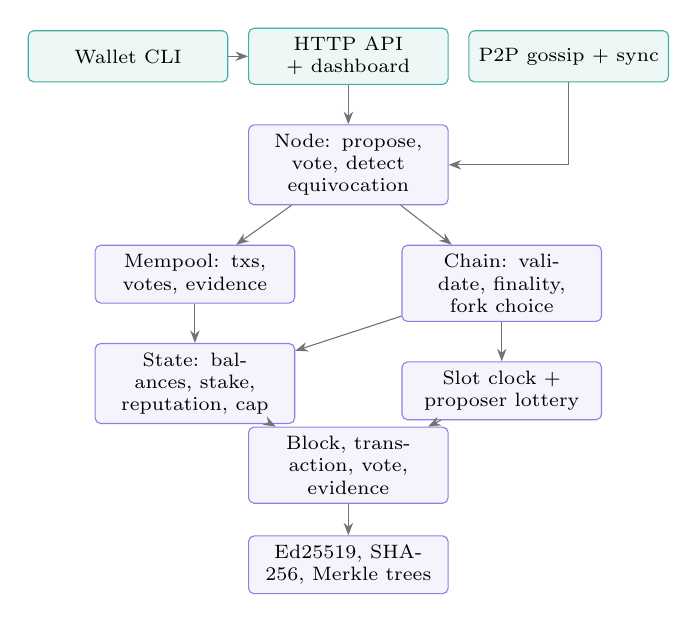
\begin{tikzpicture}[
  box/.style={draw=nyx!70,fill=nyx!6,rounded corners=2pt,minimum height=6.5mm,text width=2.3cm,align=center,font=\scriptsize},
  io/.style={draw=nyx2!80,fill=nyx2!8,rounded corners=2pt,minimum height=6.5mm,text width=2.3cm,align=center,font=\scriptsize},
  arr/.style={-{Stealth[length=1.6mm]},draw=black!55}]
\node[io] (api) {HTTP API + dashboard};
\node[io,left=0.25cm of api] (cli) {Wallet CLI};
\node[io,right=0.25cm of api] (p2p) {P2P gossip + sync};
\node[box,below=0.5cm of api] (node) {Node: propose, vote, detect equivocation};
\node[box,below left=0.5cm and -0.6cm of node] (mem) {Mempool: txs, votes, evidence};
\node[box,below right=0.5cm and -0.6cm of node] (chain) {Chain: validate, finality, fork choice};
\node[box,below=0.5cm of mem] (state) {State: balances, stake, reputation, cap};
\node[box,below=0.5cm of chain] (cons) {Slot clock + proposer lottery};
\node[box,below=0.5cm of $(state)!0.5!(cons)$] (data) {Block, transaction, vote, evidence};
\node[box,below=0.4cm of data] (crypto) {Ed25519, SHA-256, Merkle trees};
\draw[arr] (cli) -- (api);
\draw[arr] (api) -- (node);
\draw[arr] (p2p) |- (node);
\draw[arr] (node) -- (mem);
\draw[arr] (node) -- (chain);
\draw[arr] (chain) -- (cons);
\draw[arr] (chain) -- (state);
\draw[arr] (mem) -- (state);
\draw[arr] (state) -- (data);
\draw[arr] (cons) -- (data);
\draw[arr] (data) -- (crypto);
\end{tikzpicture}
\caption{Layers of a NyxChain node. Teal components face the outside world; purple components form the protocol core.}
\label{fig:arch}
\end{figure}

\subsection{Data Structures}
A \emph{transaction} carries its kind (transfer, stake or unstake), the sender's public key, recipient, amount, fee, a per-account nonce and an Ed25519 signature. The sender's address is derived from its public key, so a transaction cannot claim another account, and the nonce must equal the number of transactions previously sent, which makes every transaction single-use. A \emph{block} header holds the height, the parent hash, the slot, a timestamp, the proposer's public key and a body root: a Merkle root over the Merkle roots of the block's transactions, finality votes and slashing evidence. The proposer signs the header, so a single signature commits to the entire block. A \emph{vote} is a signed statement that a validator accepts a given block at a given height. \emph{Evidence} is a pair of signed messages from one validator that cannot both be honest: two votes at one height for different blocks, or two block headers for one slot.

\subsection{Block Lifecycle}
Fig.~\ref{fig:lifecycle} shows the path of a block from proposal to finality.

\begin{figure*}[t]
\centering
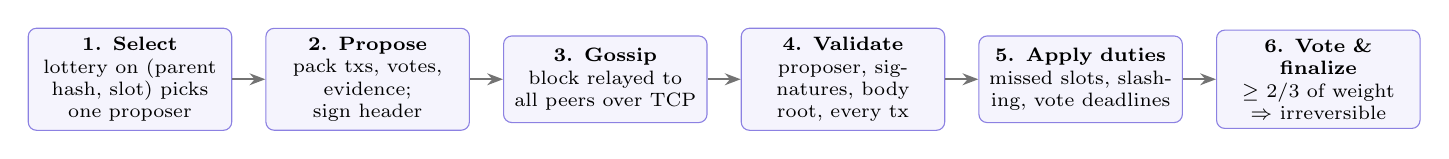
\begin{tikzpicture}[
  st/.style={draw=nyx!70,fill=nyx!6,rounded corners=3pt,minimum height=11mm,text width=2.35cm,align=center,font=\scriptsize},
  arr/.style={-{Stealth[length=2mm]},draw=black!55,thick}]
\node[st] (a) {\textbf{1. Select}\\lottery on (parent hash, slot) picks one proposer};
\node[st,right=0.42cm of a] (b) {\textbf{2. Propose}\\pack txs, votes, evidence; sign header};
\node[st,right=0.42cm of b] (c) {\textbf{3. Gossip}\\block relayed to all peers over TCP};
\node[st,right=0.42cm of c] (d) {\textbf{4. Validate}\\proposer, signatures, body root, every tx};
\node[st,right=0.42cm of d] (e) {\textbf{5. Apply duties}\\missed slots, slashing, vote deadlines};
\node[st,right=0.42cm of e] (f) {\textbf{6. Vote \& finalize}\\$\geq$ 2/3 of weight $\Rightarrow$ irreversible};
\draw[arr] (a) -- (b); \draw[arr] (b) -- (c); \draw[arr] (c) -- (d); \draw[arr] (d) -- (e); \draw[arr] (e) -- (f);
\end{tikzpicture}
\caption{Block lifecycle. Steps 1 and 4--6 are computed identically by every node from public data, so no extra messages are needed to agree on the proposer, on penalties or on finality.}
\label{fig:lifecycle}
\end{figure*}

\subsection{Proposer Selection}
Time is divided into slots of fixed length. Each validator $v$ with stake $s_v \geq 100$ and reputation $r_v \in [0,1]$ has raw weight $\hat w_v = \lfloor s_v r_v \rfloor$ and voting weight $w_v$, obtained from $\hat w_v$ by the cap of Section~\ref{sec:cap}. For slot $t$ on parent block $P$, every node computes
\begin{equation}
x = \mathrm{SHA256}\big(\mathrm{hash}(P)\,\|\,t\big) \bmod W, \qquad W = \textstyle\sum_v w_v,
\end{equation}
and selects the validator at which the cumulative weight, taken in a fixed order, first exceeds $x$. The probability of selection is $w_v/W$, and because the inputs are public every node reaches the same result without communication. If the selected validator is absent, the slot remains empty and the next slot selects again.

\subsection{Reputation as Recent Reliability}
Each duty a validator performs is one sample $o \in \{0,1\}$ in an exponentially weighted moving average,
\begin{equation}
r_v \leftarrow d\, r_v + (1-d)\, o, \qquad d = 0.9862,
\label{eq:ewma}
\end{equation}
so a sample loses half of its influence after $\ln 0.5/\ln d \approx 50$ newer samples. Reputation is stored in basis points and computed as a contraction of the gap to 100\% on success, or to 0\% on failure, which is algebraically identical to (\ref{eq:ewma}) but remains exact in integer arithmetic. The duties are listed in Table~\ref{tab:duties}; every one is verifiable from the chain, so all nodes compute identical scores. A floor of 5\% guarantees that a validator returning from an outage can still vote and recover.

\begin{table}[t]
\centering
\caption{Reputation Duties and Initial Values}
\label{tab:duties}
\footnotesize
\begin{tabularx}{\columnwidth}{@{}L{3.1cm} L{1.5cm} Y@{}}
\toprule
\textbf{Event} & \textbf{Samples} & \textbf{Rationale}\\
\midrule
Vote for block $h$ recorded by block $h{+}3$ & 1 success or 1 failure & Every validator, every block; deadline absorbs delay\\
Proposes a block when selected & 1 success & Performing the role\\
Selected for a slot and absent & 5 failures & A missed block costs the whole network a slot\\
\midrule
Genesis validator & starts at 50\% & ---\\
Validator staking later & starts at 10\% & Influence is not bought at once\\
Proven equivocation & set to 0, excluded & Section~\ref{sec:slash}\\
\bottomrule
\end{tabularx}
\end{table}

Three properties follow. Validators that perform all duties converge to the same reputation regardless of their starting value, so early arrival confers no lasting advantage. A validator that stops contributing loses its standing irrespective of its history. A crashed validator regains standing at the same rate once it returns. Duties are charged only from the height at which a validator joined, so a newcomer is never debited for blocks that preceded it, and votes for already-finalized blocks still earn their author credit, so a validator whose vote arrives just after finality is not treated as late.

\subsection{Bounded Voting-Weight Cap}\label{sec:cap}
Equal reputation transfers control to stake. A cap therefore reduces the largest validators so that none holds more than 30\% of voting weight. If the $k$ largest validators are capped at $c$ and the remainder sum to $R$, then $c = 0.3(kc + R)$, giving
\begin{equation}
c_{\mathrm{wf}} = \frac{0.3\,R}{1 - 0.3\,k},
\label{eq:wf}
\end{equation}
taken for the smallest $k$ at which $c_{\mathrm{wf}}$ lies between the $k$-th and $(k{+}1)$-th largest raw weights.

Capping a validator raises every other validator's share by the factor $\hat W / W$. When only one or two validators are large, (\ref{eq:wf}) alone hands most of the vote to whoever else is present. The cap is therefore raised, when required, to the smallest value $c$ satisfying
\begin{equation}
\textstyle\sum_v \min(\hat w_v, c) \;\geq\; \hat W / 2,
\label{eq:boost}
\end{equation}
so that no validator's share is ever more than doubled. The final cap is $\max(c_{\mathrm{wf}}, c)$. Validators below the cap are unaffected. A single validator is held to 30\% while it owns less than approximately 65\% of raw weight; above that point enforcing 30\% would violate (\ref{eq:boost}), so the cap reduces the validator by less. With three or fewer validators a 30\% limit could only be met by equalizing all weights, so the cap applies from four validators upward.

The value of 30\% is chosen relative to finality. Because finality requires two thirds of weight, it stalls only when more than one third is absent or abstains; a validator below one third cannot stall finality alone.

\subsection{Two-Thirds Finality and Fork Choice}
After accepting a new block, each validator signs a vote for it, at most once per height; the last voted height is persisted so that a restart cannot produce an accidental double vote. Votes are gossiped and included in subsequent blocks. A vote is counted only if it targets an ancestor of the including block within a 64-block window, is correctly signed, comes from an active validator and has not been counted before. When the counted votes for block $B$ satisfy
\begin{equation}
3 \textstyle\sum_{v \in \mathrm{voters}(B)} w_v \;\geq\; 2W,
\end{equation}
$B$ and its ancestors become final, and a node refuses any block that does not descend from its finalized block. Under the standard assumption that less than one third of weight is Byzantine, two conflicting blocks cannot both gather two-thirds support without one third of weight voting twice. Competing branches are ordered by finalized height, then length, then lowest tip hash.

\subsection{Accountability: Slashing and Unbonding}\label{sec:slash}
A node receiving two conflicting signed messages from one validator constructs evidence and gossips it; the next proposer includes it. The offender loses half of its stake and of any coins it is unbonding, of which 10\% is paid to the including proposer and 90\% is destroyed; its reputation is set to zero and it may never stake again. Unstaked coins remain locked, and slashable, for ten blocks, so a validator cannot misbehave and withdraw before evidence is recorded.

\subsection{Networking and Persistence}
A node dials every peer it knows and accepts inbound connections. The \texttt{hello} message carries the node's height, finalized height and known peers, so a node configured with one seed discovers the rest. A node that is behind requests blocks from its finalized height onward. Peer discovery follows the contact-learning principle of Kademlia \cite{maymounkov2002}, in simplified form. Dead peers are redialled every two seconds, and every accepted block is appended to disk, so a restarted node reloads its history and synchronizes only the remainder.

\subsection{Evaluation Metrics}
Table~\ref{tab:metrics} defines the evaluators used in Section~\ref{sec:results}.

\begin{table}[t]
\centering
\caption{Performance Evaluators}
\label{tab:metrics}
\footnotesize
\begin{tabularx}{\columnwidth}{@{}L{2.2cm} Y@{}}
\toprule
\textbf{Evaluator} & \textbf{Definition}\\
\midrule
Throughput & Transfers included per second over the slots that carried the load\\
Finality latency & Time from the first observation of a block to the first observation of its finality\\
Recovery time & Time from restart of a crashed node until it is within one block of the network\\
Liveness under fault & Growth of block and finalized height while a validator is offline\\
Reputation spread & Largest minus smallest reputation among validators performing equal work\\
Voting share & A validator's capped weight divided by total capped weight\\
Agreement & Identical block hash at the minimum finalized height on every node\\
\bottomrule
\end{tabularx}
\end{table}

\subsection{Verification Provisions}
Each property in Table~\ref{tab:targets} is expressed as an executable check fixed before the corresponding run; scripts exit with a failure status if any check is not met. The cap was additionally examined with randomized inputs, and the complete implementation was subjected to an independent code review, whose findings are reported in Section~\ref{sec:review}.

%=====================================================================
\section{Experimental Results and Discussion}\label{sec:results}

\subsection{Experimental Setup}
All runs used the configurations of Table~\ref{tab:configs} on a single two-core host with Python~3.13. The unit tests were executed 20 times consecutively without failure. Each end-to-end and attack scenario was run on a freshly generated network, and the outputs, node logs and dashboard screenshots reported below are those of the recorded runs.

\subsection{Correctness}
Table~\ref{tab:unit} summarizes the 30 unit tests, all of which pass. In addition, the cap was evaluated on 100{,}000 random weight lists of one to twelve validators: in every case no weight was increased, order was preserved, every weight remained positive, no share was more than doubled, and, with five or more validators, a single dominant validator owning less than 64\% of raw weight was held to 30\%.

\begin{table}[t]
\centering
\caption{Unit Test Coverage (30/30 Passed)}
\label{tab:unit}
\footnotesize
\begin{tabularx}{\columnwidth}{@{}L{1.7cm} Y@{}}
\toprule
\textbf{Area} & \textbf{Properties tested}\\
\midrule
Transactions & Tampering detected; replayed nonce and overspending rejected\\
State & Late stakers start at 10\%; unbonding returns coins after 10 blocks; supply conserved\\
Blocks & Wrong proposer, altered contents and future blocks rejected\\
Reputation & Halves after 50 failures; reaches exactly 100\%; floor of 5\%; newcomer and founders within 3 points after equal work; history does not protect a quitter; vote deadline; no duties before joining\\
Cap & Whale held to 30\%; several whales; no cap with 3 validators; small or crashed validators never boosted beyond 2$\times$; lottery and finality use capped weight\\
Finality & One third does not finalize, two thirds does; forged, outsider and duplicate votes rejected; conflicting branch refused\\
Slashing & Double vote and double block slashed; no double slashing; forged evidence rejected\\
Fork choice & Longer branch preferred; more-finalized branch beats longer branch\\
\bottomrule
\end{tabularx}
\end{table}

\subsection{End-to-End Behaviour}
Table~\ref{tab:demo} reports the 20 checks of the end-to-end scenario, all of which passed. Every node discovered all three peers from a single seed; blocks were finalized from the first seconds; and the four nodes agreed exactly on account balances after transfers and staking.

\begin{table}[t]
\centering
\caption{End-to-End Scenario (20/20 Checks Passed)}
\label{tab:demo}
\footnotesize
\begin{tabularx}{\columnwidth}{@{}L{1.3cm} Y L{1.8cm}@{}}
\toprule
\textbf{Stage} & \textbf{Check} & \textbf{Measured}\\
\midrule
Start & Peers discovered from one seed & 3/3 per node\\
 & Blocks finalized by 2/3 votes & height 7, final 6\\
Wallet & Nodes agree on balances & 949 on all 4\\
 & New staker joins low & 10\% vs 50\%\\
 & Unstaked coins locked & 100 unbonding\\
Crash & Chain grows without node3 & +18 in 20 slots\\
 & Finality continues & 16 $\to$ 34\\
 & node3 reputation falls & 60\% $\to$ 43\%\\
Restart & Catches up from disk & all at 38\\
Reputation & Equal work, equal score & 75, 73, 75\%\\
 & Idle staker fades & 10\% $\to$ 7\%\\
Whale & Share capped & 40\% $\to$ 29.99\%\\
 & Finality continues & 39 $\to$ 46\\
End & Unbonded coins released & 948 $\to$ 1048\\
 & Identical finalized block & \#47 on all 4\\
 & Honest blocks rejected & 0\\
\bottomrule
\end{tabularx}
\end{table}

\subsection{Crash Fault Tolerance}
When a validator was terminated, the remaining three continued to produce and finalize blocks; the absent validator's reputation fell with every missed duty, reducing its selection probability, and after restart it reloaded its blocks from disk and synchronized the remainder (Fig.~\ref{fig:recovery}). In the benchmark run, 13 blocks were produced during a 15\,s outage, the crashed validator's reputation fell from 62\% to 48\%, and it was back within one block of the network 0.71\,s after restart.

\begin{figure}[t]
\centering
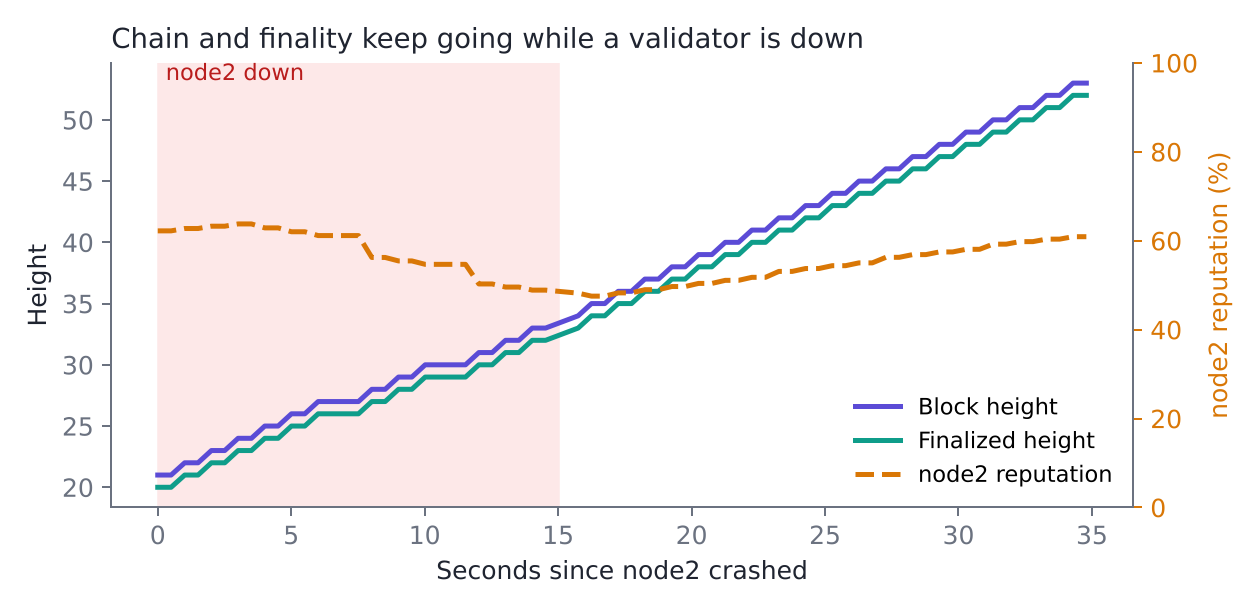
\includegraphics[width=\columnwidth]{fig/fig_recovery.png}
\caption{Crash recovery. Block height and finalized height continue to rise in step while node2 is offline (shaded); its reputation falls with each missed duty and recovers after restart.}
\label{fig:recovery}
\end{figure}

\subsection{Reputation Dynamics}
Fig.~\ref{fig:rep} shows a deterministic 300-block simulation executed through the same chain code. The newcomer, starting at 10\%, came within 3 points of the founder by block 160 and ended at 99.8\% against the founder's 100\%. The quitter, at 96.6\% when it stopped, fell below 50\% within 16 blocks and below 10\% within 98 blocks. The crashed validator dropped to 27\% during its outage and ended at 96.5\%. The validator missing about three duties in ten settled at 56\%, lower than its attendance rate because each missed slot counts five times. In the live scenario, the three running validators finished within 1.8 points of one another, while the idle staker fell from 10\% to 7\%.

\begin{figure}[t]
\centering
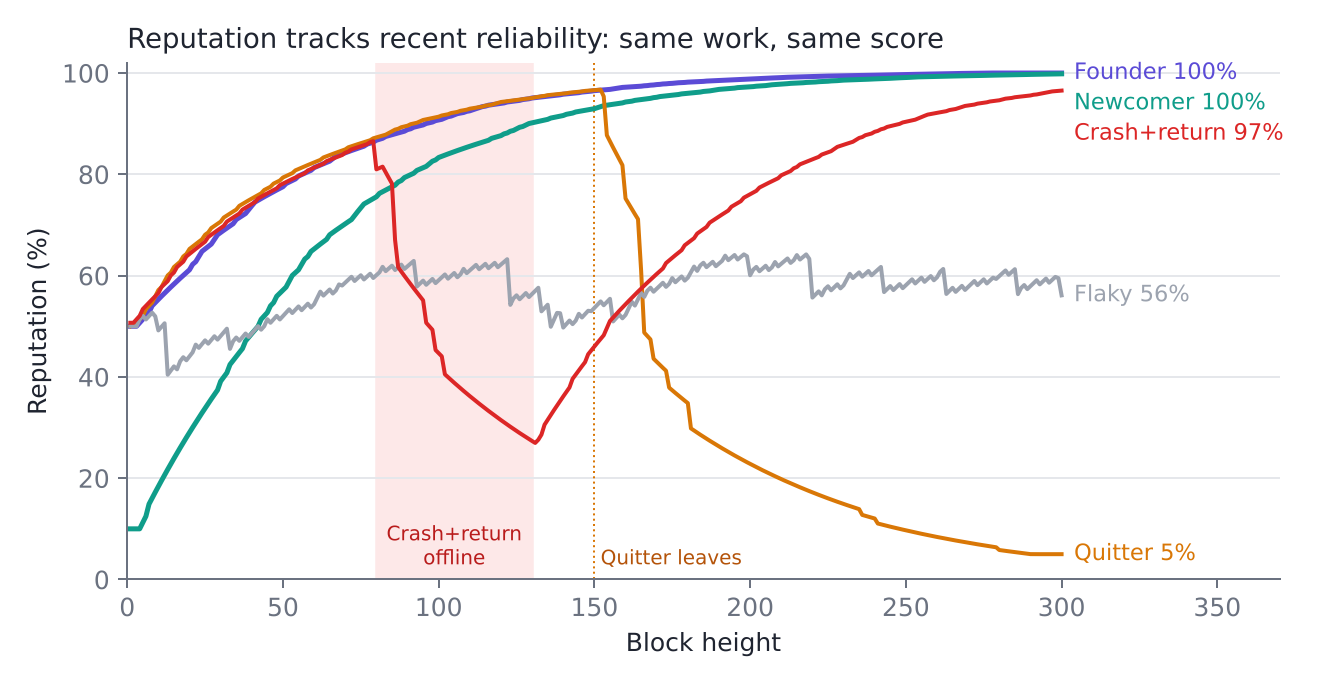
\includegraphics[width=\columnwidth]{fig/fig_reputation.png}
\caption{Reputation over 300 blocks for five behaviours. Equal work yields equal reputation; a long record does not protect a validator that stops.}
\label{fig:rep}
\end{figure}

\subsection{Voting-Weight Cap}
In the whale stage, an account staking 9{,}000 tokens at 10\% reputation held 40\% of raw weight; the cap reduced it to 29.99\%. Together with the idle staker, the offline weight would have been 40\% without the cap, above the one-third threshold at which finality stalls, and was 31\% with it; finality advanced from height 39 to 46 during the stage (Fig.~\ref{fig:whale}). Fig.~\ref{fig:cap} shows the cap's response as a validator's raw share grows: its voting share is held at 30\% until it owns about 65\% of raw weight, after which the boost limit (\ref{eq:boost}) loosens the cap.

\begin{figure}[t]
\centering
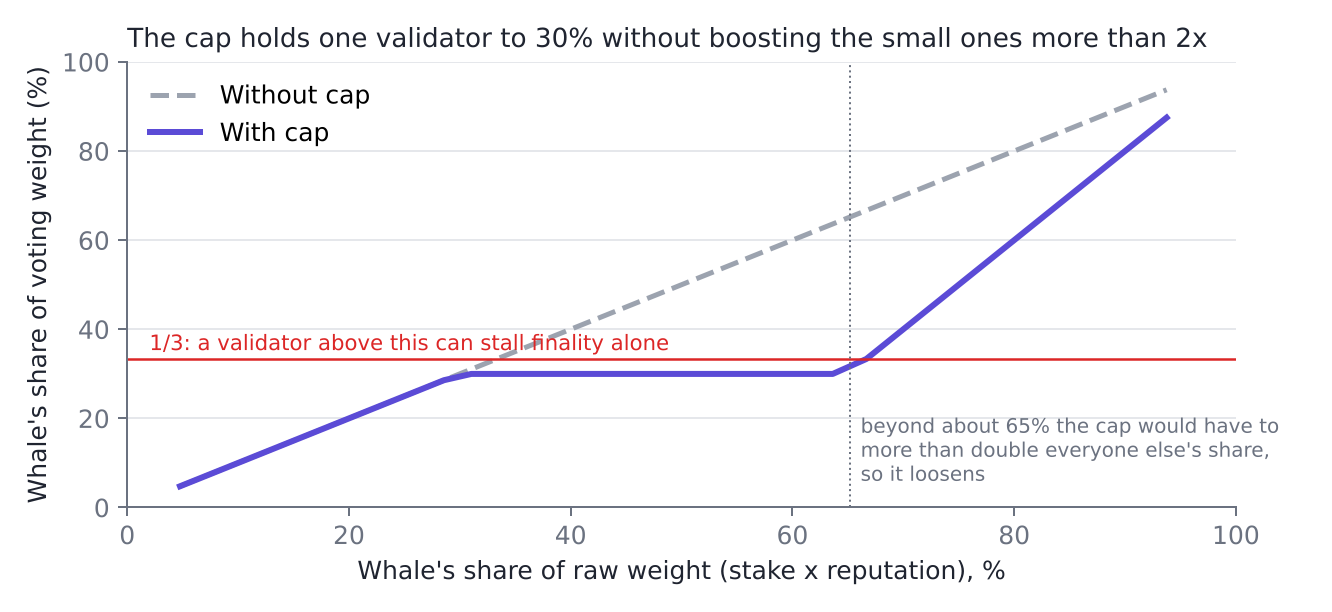
\includegraphics[width=\columnwidth]{fig/fig_cap.png}
\caption{Voting share of one validator against its share of raw weight, with four other validators at equal reputation.}
\label{fig:cap}
\end{figure}

\begin{figure*}[t]
\centering
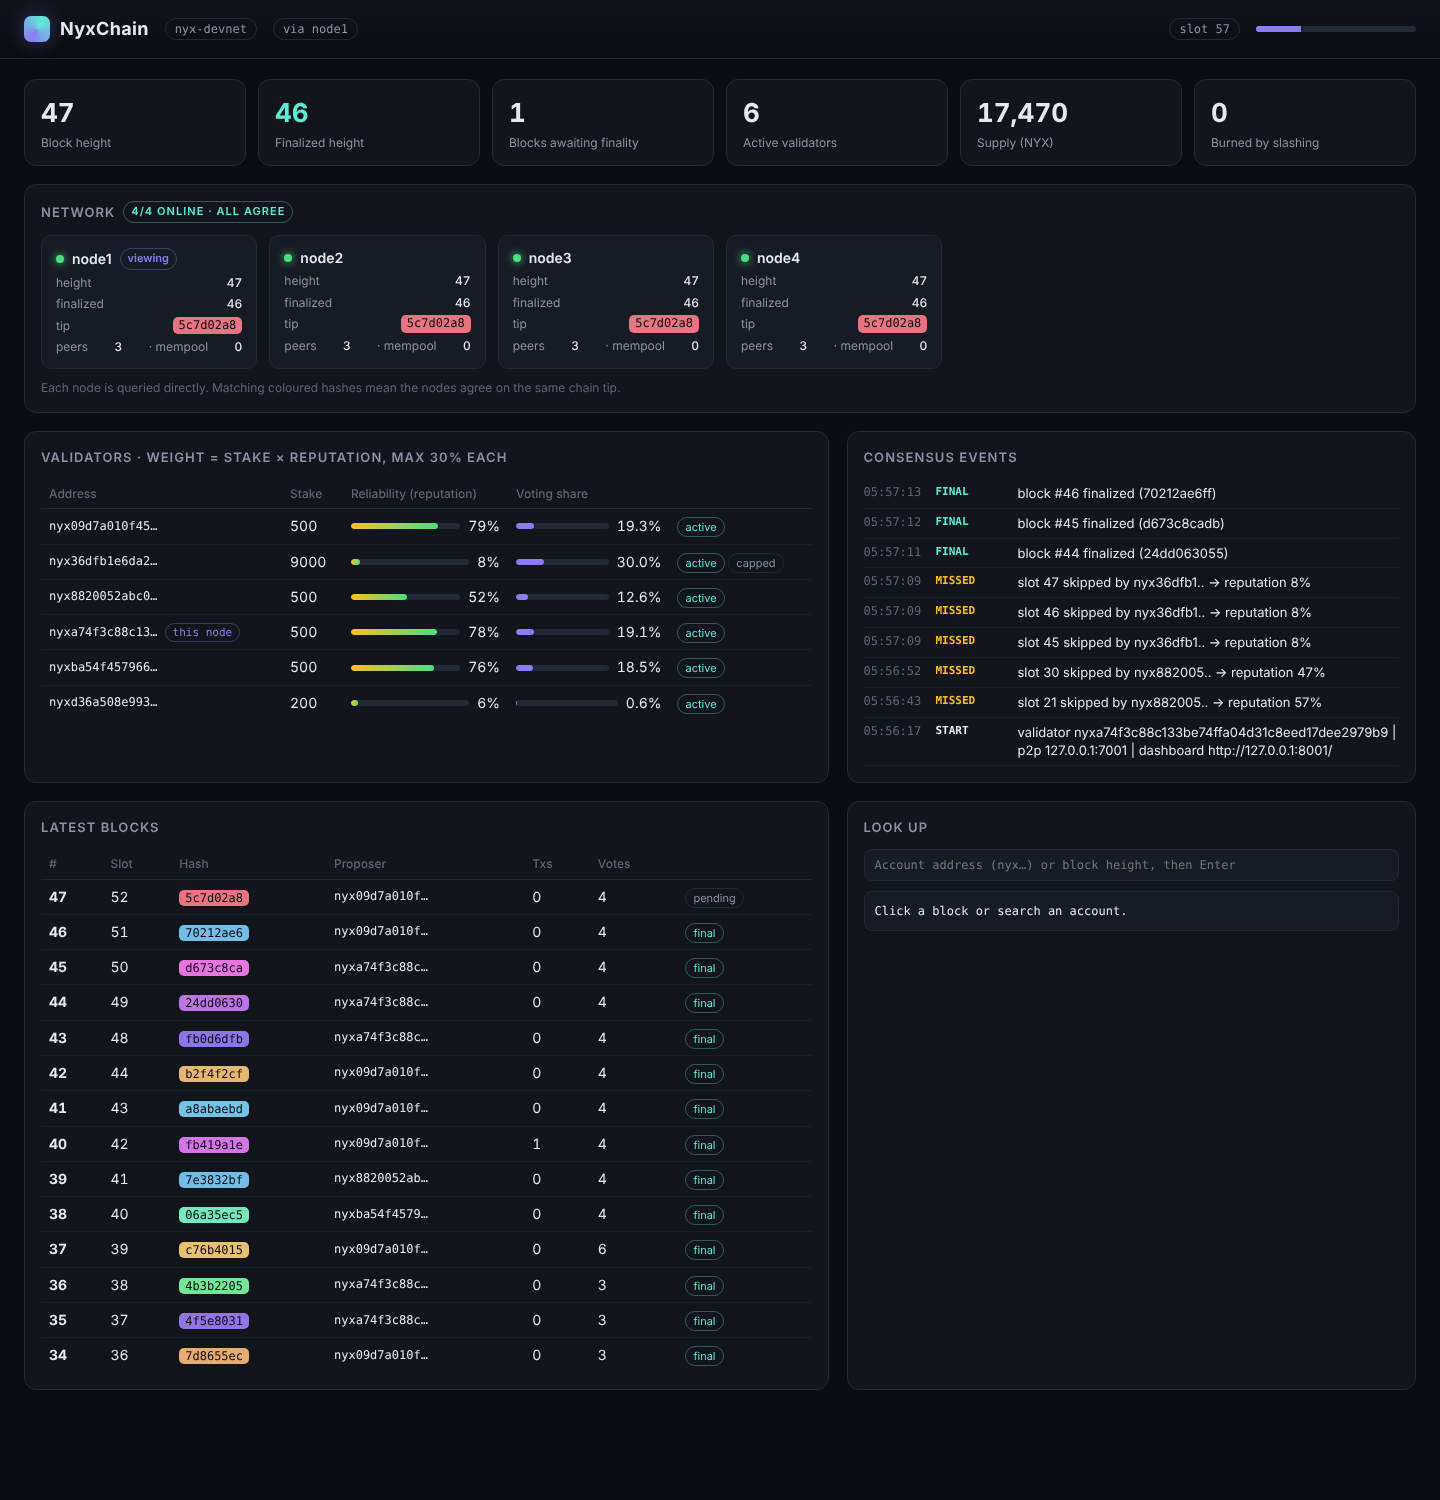
\includegraphics[width=0.49\textwidth]{fig/04_whale_capped.png}\hfill
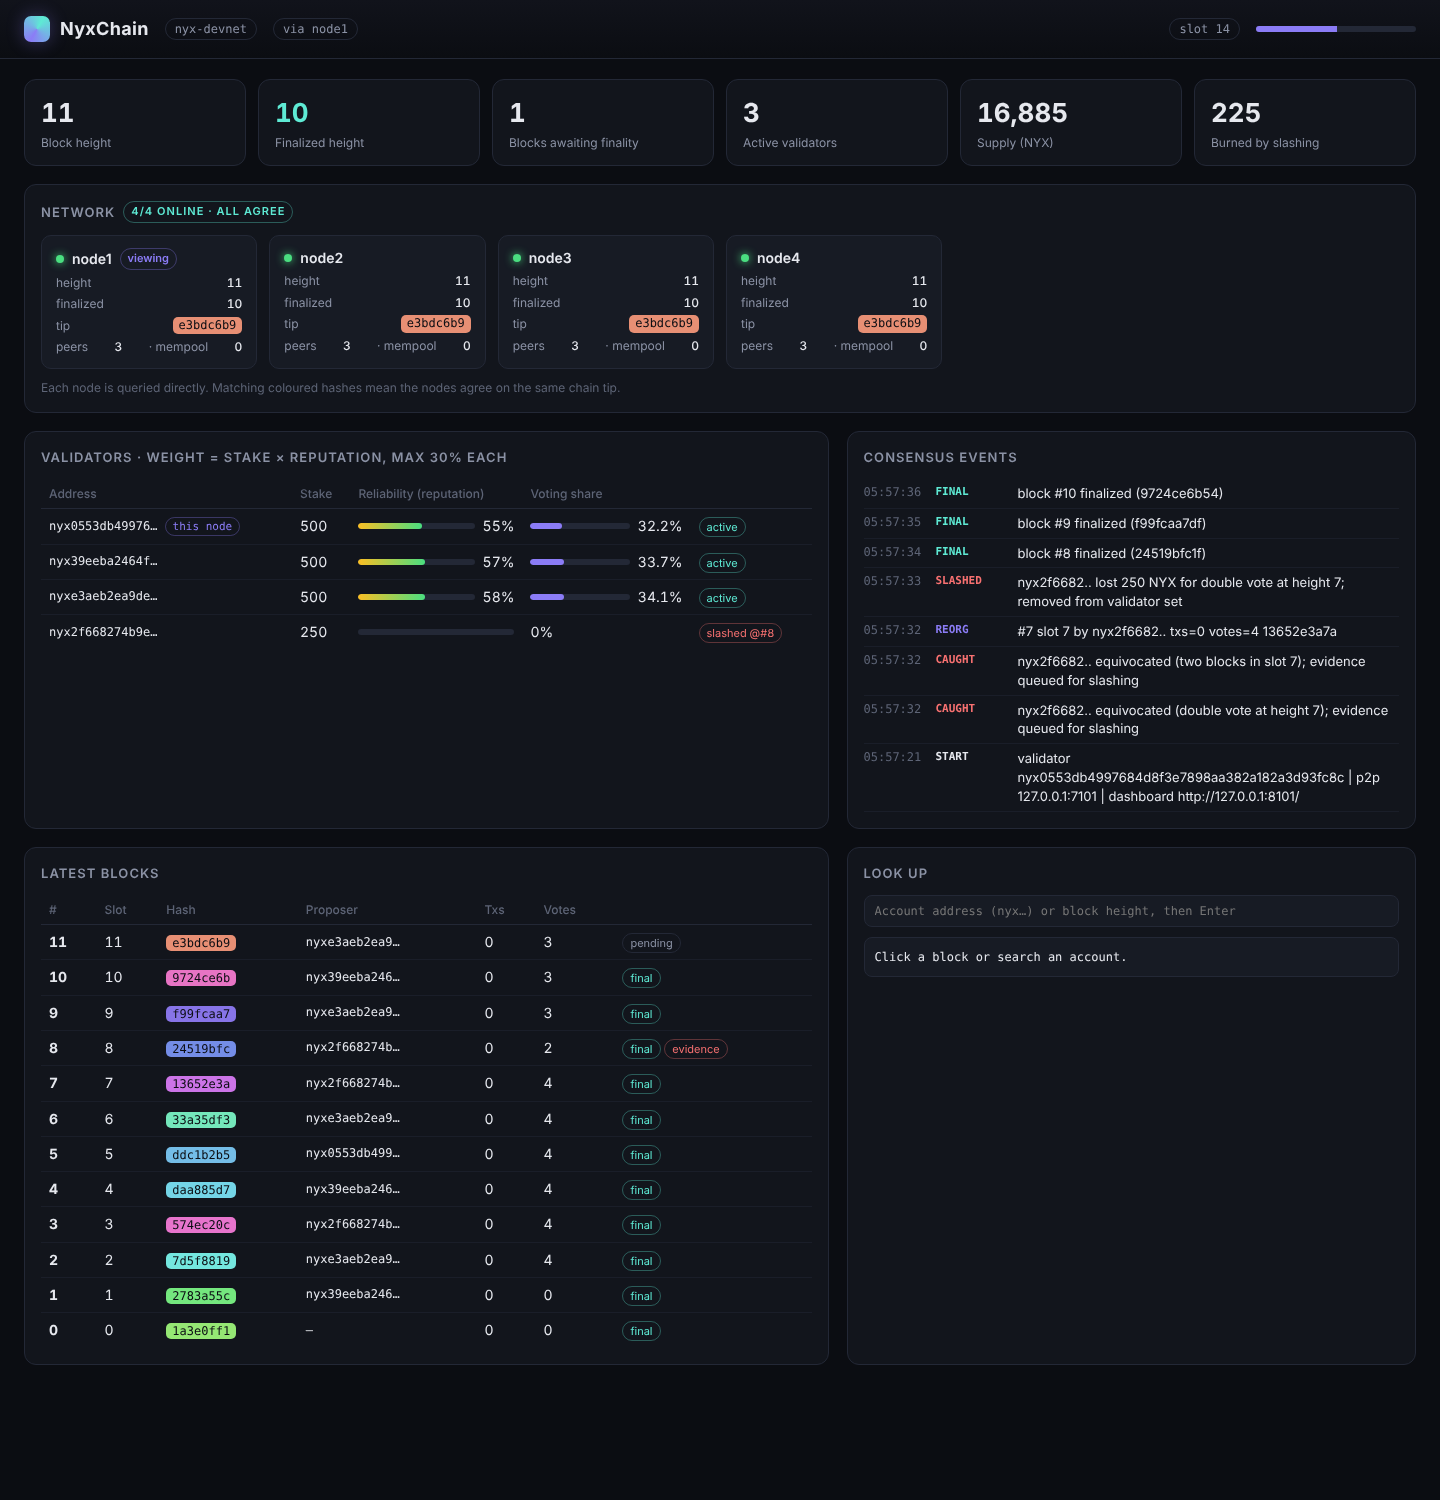
\includegraphics[width=0.49\textwidth]{fig/05_byzantine_slashed.png}
\caption{Live dashboard. Left: the offline whale (9{,}000 stake, 8\% reputation) is marked \emph{capped} at a 30.0\% share while every block is finalized one block behind the tip. Right: after the equivocation attack, the event feed shows the offence caught and slashed, the offender holds 250 stake with no voting share, and 225 tokens are burned.}
\label{fig:whale}
\end{figure*}

\subsection{Byzantine Behaviour}
In the attack scenario the Byzantine validator, selected for slot 7, signed two blocks and sent each to a different half of the network while voting for both. All three honest nodes detected both forms of equivocation within one second, and the next honest block (height 8) carried the proof. The offender's stake fell from 500 to 250, 225 tokens were destroyed and 25 paid to the reporting proposer, and it was removed from the validator set. The remaining validators continued to finalize (height 11 to 21), and all four nodes, including the offender, held the identical block at height 21, so no conflicting block was ever finalized.

\subsection{Throughput and Finality Latency}
Table~\ref{tab:perf} reports the benchmark. Throughput is bounded by design rather than by the node: under Load B every block was filled to the 500-transaction limit, so the network cleared one full block per one-second slot (Fig.~\ref{fig:tput}). Across 50 blocks, finality followed a block by a median of 1.0\,s (90th percentile 1.03\,s, maximum 2.0\,s), because the votes for block $h$ are included in block $h{+}1$ (Fig.~\ref{fig:final}); the maximum occurred while a validator was offline and its slot remained empty.

\begin{table}[t]
\centering
\caption{Benchmark Results}
\label{tab:perf}
\footnotesize
\begin{tabular}{@{}lrr@{}}
\toprule
\textbf{Metric} & \textbf{Load A} & \textbf{Load B}\\
\midrule
Transfers / sending accounts & 1{,}000 / 20 & 4{,}000 / 80\\
Blocks needed & 2 & 9\\
Throughput (transfers/s) & 509 & 446\\
Submission to all included (s) & 1.6 & 8.9\\
\midrule
Finality latency, median / p90 / max & \multicolumn{2}{c}{1.0 / 1.03 / 2.0\,s (50 blocks)}\\
Blocks produced during 15\,s outage & \multicolumn{2}{c}{13}\\
Recovery after restart & \multicolumn{2}{c}{0.71\,s}\\
\bottomrule
\end{tabular}
\end{table}

\begin{figure}[t]
\centering
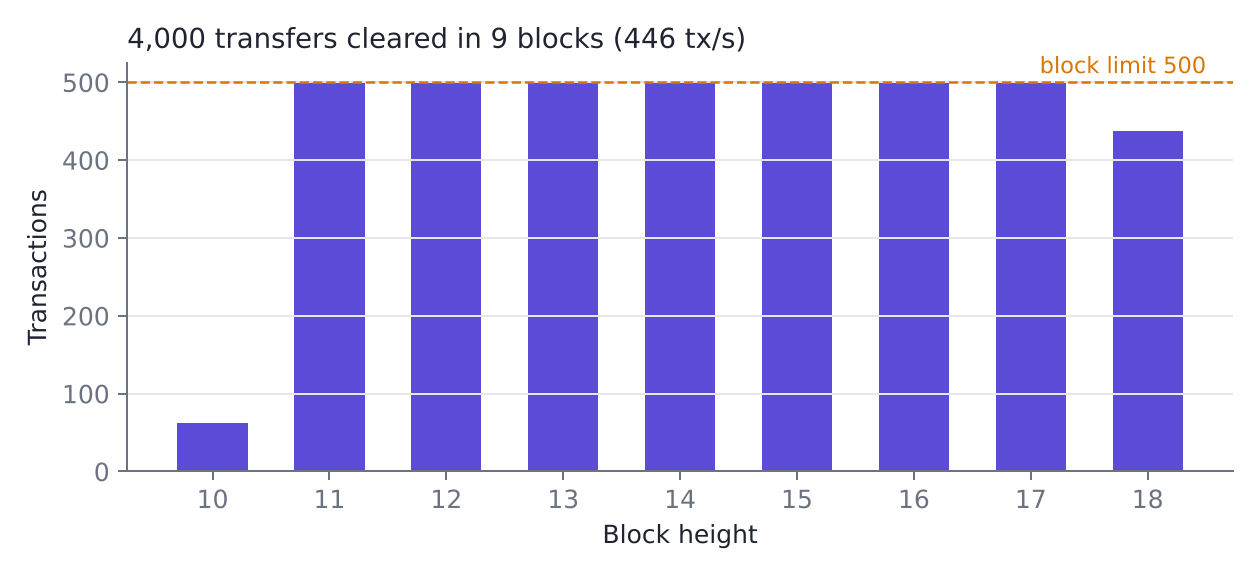
\includegraphics[width=\columnwidth]{fig/fig_throughput.png}
\caption{Transactions per block under Load B. Every block reaches the 500-transaction limit.}
\label{fig:tput}
\end{figure}

\begin{figure}[t]
\centering
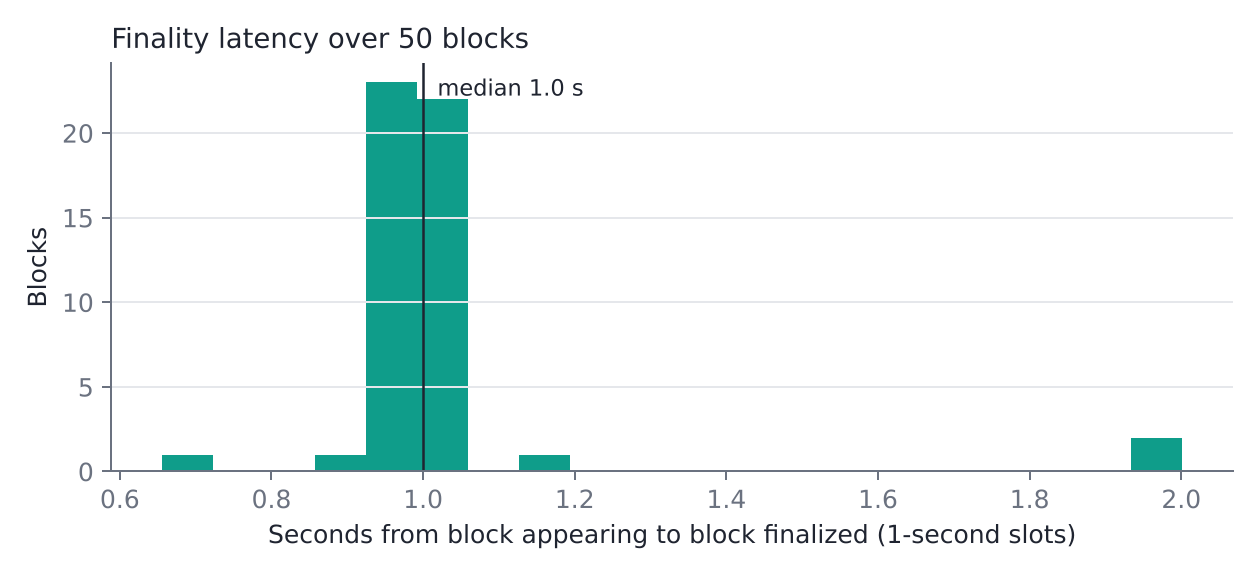
\includegraphics[width=\columnwidth]{fig/fig_finality.png}
\caption{Distribution of finality latency over 50 blocks with one-second slots.}
\label{fig:final}
\end{figure}

\subsection{Independent Code Review}\label{sec:review}
After the reputation rule and the cap were implemented, the code was examined by an independent reviewer who had not taken part in writing it, with instructions to reproduce any suspected fault. Table~\ref{tab:review} lists the findings. The most consequential concerned the first formulation of the cap, which used water-filling (\ref{eq:wf}) alone: two validators of 100 tokens beside two of 100{,}000 received 40\% of the vote, and a crashed validator at the 5\% floor was restored to the same weight as healthy ones. Under the boost limit (\ref{eq:boost}) the same cases yield 0.03\% for the two small validators combined and 4.9\% for the crashed validator; all three cases are retained as regression tests. The reviewer found no source of non-determinism between nodes and no way for a vote to be counted twice.

\begin{table}[t]
\centering
\caption{Code Review Findings and Resolutions}
\label{tab:review}
\footnotesize
\begin{tabularx}{\columnwidth}{@{}Y Y@{}}
\toprule
\textbf{Finding} & \textbf{Resolution}\\
\midrule
Water-filling alone gives small or crashed validators decisive weight & Boost limit (\ref{eq:boost}); regression tests\\
Newcomers charged for blocks before joining & Activation height recorded\\
Counted votes dropped before a reorganization & Retained until outside the window\\
Integer rounding capped reputation at 99.28\% & Gap-contraction form; reaches 100\%\\
A demonstration claim depended on run-time numbers & Computed and printed per run\\
Cap test did not exercise lottery or finality & Extended to both\\
Honest validator may lose one sample after a reorganization; grandparent reorganizations possible & Documented as limitations\\
\bottomrule
\end{tabularx}
\end{table}

\subsection{Computational Cost}
Table~\ref{tab:cost} lists wall-clock times for each verification stage on the two-core host.

\begin{table}[t]
\centering
\caption{Computational Cost (Single Host, 2 CPU Cores)}
\label{tab:cost}
\footnotesize
\begin{tabular}{@{}lr@{}}
\toprule
\textbf{Stage} & \textbf{Wall time}\\
\midrule
Unit tests (30) & 0.6\,s\\
Reputation simulation (300 blocks) & 5\,s\\
Attack scenario (4 processes) & 40\,s\\
End-to-end scenario (4 processes) & 2\,min\\
Benchmark (4 processes, 5{,}000 transfers) & 2\,min\\
\bottomrule
\end{tabular}
\end{table}

\subsection{Limitations}
Six limitations qualify the results. First, all nodes ran on one machine, so network latency is close to zero and the throughput figures reflect validation cost rather than propagation. Second, finality uses a single voting round; Casper FFG uses two rounds (justification and finalization) to remain safe under weaker assumptions about honest voting \cite{buterin2017}. Third, the cap cannot restrain a participant owning most of all stake and behaving reliably; above about 65\% of raw weight it loosens rather than inflate every other participant. Fourth, after a reorganization an honest validator that has already voted at that height loses one reputation sample, and a proposer can build on its grandparent to orphan a rival's block when the hash tie-break favours it. Fifth, block headers carry no state root, so a divergence between nodes would go undetected; the review found no source of divergence, but a state root would make this verifiable. Sixth, slot timing assumes clocks synchronized to within about one second.

%=====================================================================
\section{Conclusion}
This study built and evaluated NyxChain, a Layer-1 blockchain implemented from first principles, in which validator weight is the product of stake and recent reliability, a single validator's share is bounded without inflating the remainder, and blocks become irreversible once two thirds of weight has voted for them. Defining reputation as a moving average over verifiable duties made it both fair and self-correcting: validators performing equal work finished within 1.8 points of one another, a newcomer caught up with a founder, a validator with a long record lost its standing within 16 blocks of stopping, and a crashed validator recovered once it returned. The cap held an offline participant with eighteen times a regular stake to 30\% of the vote, which kept finality advancing where the uncapped configuration would have stalled it, while the boost limit ensured that small and unreliable validators were never handed decisive weight. Equivocation was detected and slashed within one block, and no conflicting block was ever finalized.

The independent review showed why the boost limit is necessary: a share cap enforced by water-filling alone transfers power to the smallest participants precisely when the network is most concentrated. The clearest next steps are two-round finality, a state root in each header, a proposer boost in fork choice to prevent grandparent reorganizations, private leader election using verifiable random functions as in Ouroboros Praos \cite{david2018}, and deployment across separate machines with simulated latency and partitions.

\begin{thebibliography}{00}
\bibitem{nakamoto2008} S. Nakamoto, ``Bitcoin: A peer-to-peer electronic cash system,'' 2008. [Online]. Available: https://bitcoin.org/bitcoin.pdf
\bibitem{garay2015} J. Garay, A. Kiayias, and N. Leonardos, ``The Bitcoin backbone protocol: Analysis and applications,'' in \textit{Proc. EUROCRYPT}, 2015, pp. 281--310.
\bibitem{eyal2014} I. Eyal and E. G. Sirer, ``Majority is not enough: Bitcoin mining is vulnerable,'' in \textit{Proc. Financial Cryptography and Data Security (FC)}, 2014, pp. 436--454.
\bibitem{kiayias2017} A. Kiayias, A. Russell, B. David, and R. Oliynykov, ``Ouroboros: A provably secure proof-of-stake blockchain protocol,'' in \textit{Proc. CRYPTO}, 2017, pp. 357--388.
\bibitem{david2018} B. David, P. Ga\v{z}i, A. Kiayias, and A. Russell, ``Ouroboros Praos: An adaptively-secure, semi-synchronous proof-of-stake blockchain,'' in \textit{Proc. EUROCRYPT}, 2018, pp. 66--98.
\bibitem{gilad2017} Y. Gilad, R. Hemo, S. Micali, G. Vlachos, and N. Zeldovich, ``Algorand: Scaling Byzantine agreements for cryptocurrencies,'' in \textit{Proc. 26th ACM Symp. Operating Systems Principles (SOSP)}, Shanghai, China, 2017, pp. 51--68.
\bibitem{buterin2017} V. Buterin and V. Griffith, ``Casper the friendly finality gadget,'' arXiv preprint arXiv:1710.09437, 2017.
\bibitem{yin2019} M. Yin, D. Malkhi, M. K. Reiter, G. Golan Gueta, and I. Abraham, ``HotStuff: BFT consensus with linearity and responsiveness,'' in \textit{Proc. ACM Symp. Principles of Distributed Computing (PODC)}, 2019, pp. 347--356.
\bibitem{yu2019} J. Yu, D. Kozhaya, J. Decouchant, and P. Esteves-Verissimo, ``RepuCoin: Your reputation is your power,'' \textit{IEEE Trans. Computers}, 2019; Cryptology ePrint Archive, Paper 2018/239.
\bibitem{aluko2021} O. Aluko and A. Kolonin, ``Proof-of-reputation: An alternative consensus mechanism for blockchain systems,'' arXiv preprint arXiv:2108.03542, 2021.
\bibitem{lamport1982} L. Lamport, R. Shostak, and M. Pease, ``The Byzantine generals problem,'' \textit{ACM Trans. Programming Languages and Systems}, vol. 4, no. 3, pp. 382--401, 1982.
\bibitem{castro1999} M. Castro and B. Liskov, ``Practical Byzantine fault tolerance,'' in \textit{Proc. 3rd USENIX Symp. Operating Systems Design and Implementation (OSDI)}, New Orleans, LA, USA, 1999, pp. 173--186.
\bibitem{ongaro2014} D. Ongaro and J. Ousterhout, ``In search of an understandable consensus algorithm,'' in \textit{Proc. USENIX Annual Technical Conf. (ATC)}, Philadelphia, PA, USA, 2014, pp. 305--319.
\bibitem{sompolinsky2015} Y. Sompolinsky and A. Zohar, ``Secure high-rate transaction processing in Bitcoin,'' in \textit{Proc. Financial Cryptography and Data Security (FC)}, 2015, pp. 507--527.
\bibitem{sompolinsky2018} Y. Sompolinsky, S. Wyborski, and A. Zohar, ``PHANTOM and GHOSTDAG: A scalable generalization of Nakamoto consensus,'' Cryptology ePrint Archive, Paper 2018/104, 2018.
\bibitem{maymounkov2002} P. Maymounkov and D. Mazi\`eres, ``Kademlia: A peer-to-peer information system based on the XOR metric,'' in \textit{Proc. 1st Int. Workshop on Peer-to-Peer Systems (IPTPS)}, Cambridge, MA, USA, 2002, pp. 53--65.
\end{thebibliography}

\end{document}
